%%% Local Variables:
%%% coding: utf-8
%%% mode: latex
%%% TeX-engine: xetex
%%% End:
\documentclass[12pt,a4paper, ngerman, oneside]{scrartcl}
\usepackage[ngerman]{babel}
\usepackage[utf8]{inputenc}
\usepackage{ucs}
\usepackage{amsmath}
\usepackage{amsfonts}
\usepackage{amssymb}
\usepackage{graphics}
\usepackage{paralist}
\usepackage{floatflt} % grafiken die vom text umflossen werden
\usepackage{gensymb} % degree symbol
\usepackage{array} % grafiken in tabellen
\usepackage[linkcolor=black]{hyperref}
\usepackage{listings} \lstset{numbers=left, numberstyle=\tiny, numbersep=5pt} \lstset{language=Java}
%% Grafiken
\usepackage[pdftex]{graphicx}
\usepackage{epsfig}
\hypersetup{%
  colorlinks=true,
}

\newcommand\blfootnote[1]{%
  \begingroup
  \renewcommand\thefootnote{}\footnote{#1}%
  \addtocounter{footnote}{-1}%
  \endgroup
}
\hypersetup{
  pdfborder = {0 0 0},
  urlbordercolor = {0 0 0},
  colorlinks = true,
  linkcolor = black,
  citecolor = black,
  filecolor = black,
  urlcolor  = black
}
% Variablen
% siehe http://tex.stackexchange.com/a/290504 option 4
\def\Tiles/{8}
\def\Rundenlimit/{20}
\def\PointsPerTile/{7}
\def\PointsPerPassenger/{7}
\def\FieldsPerTile/{20}
\def\Passagiere/{5}

\newcommand{\fieldGraphic}[2]{%
\begin{floatingfigure}[#1]{0.15\textwidth}%
  \centering
  \includegraphics[width=0.15\textwidth]{bilder/#2}%
\end{floatingfigure}%
}

\sloppy
\hyphenpenalty=100000

\usepackage{fontspec}
\setromanfont{Merriweather}
\setsansfont{Lato}
\renewcommand{\normalsize}{\fontsize{12}{18}\selectfont}


\titlehead{
  \centering
\includegraphics[width=3.5cm]{bilder/logo.png}
}
\subject{Software-Challenge 2017}
\title{Spielregeln}
\subtitle{Mississippi Queen}
\date{Stand: \today}


\begin{document}
\maketitle
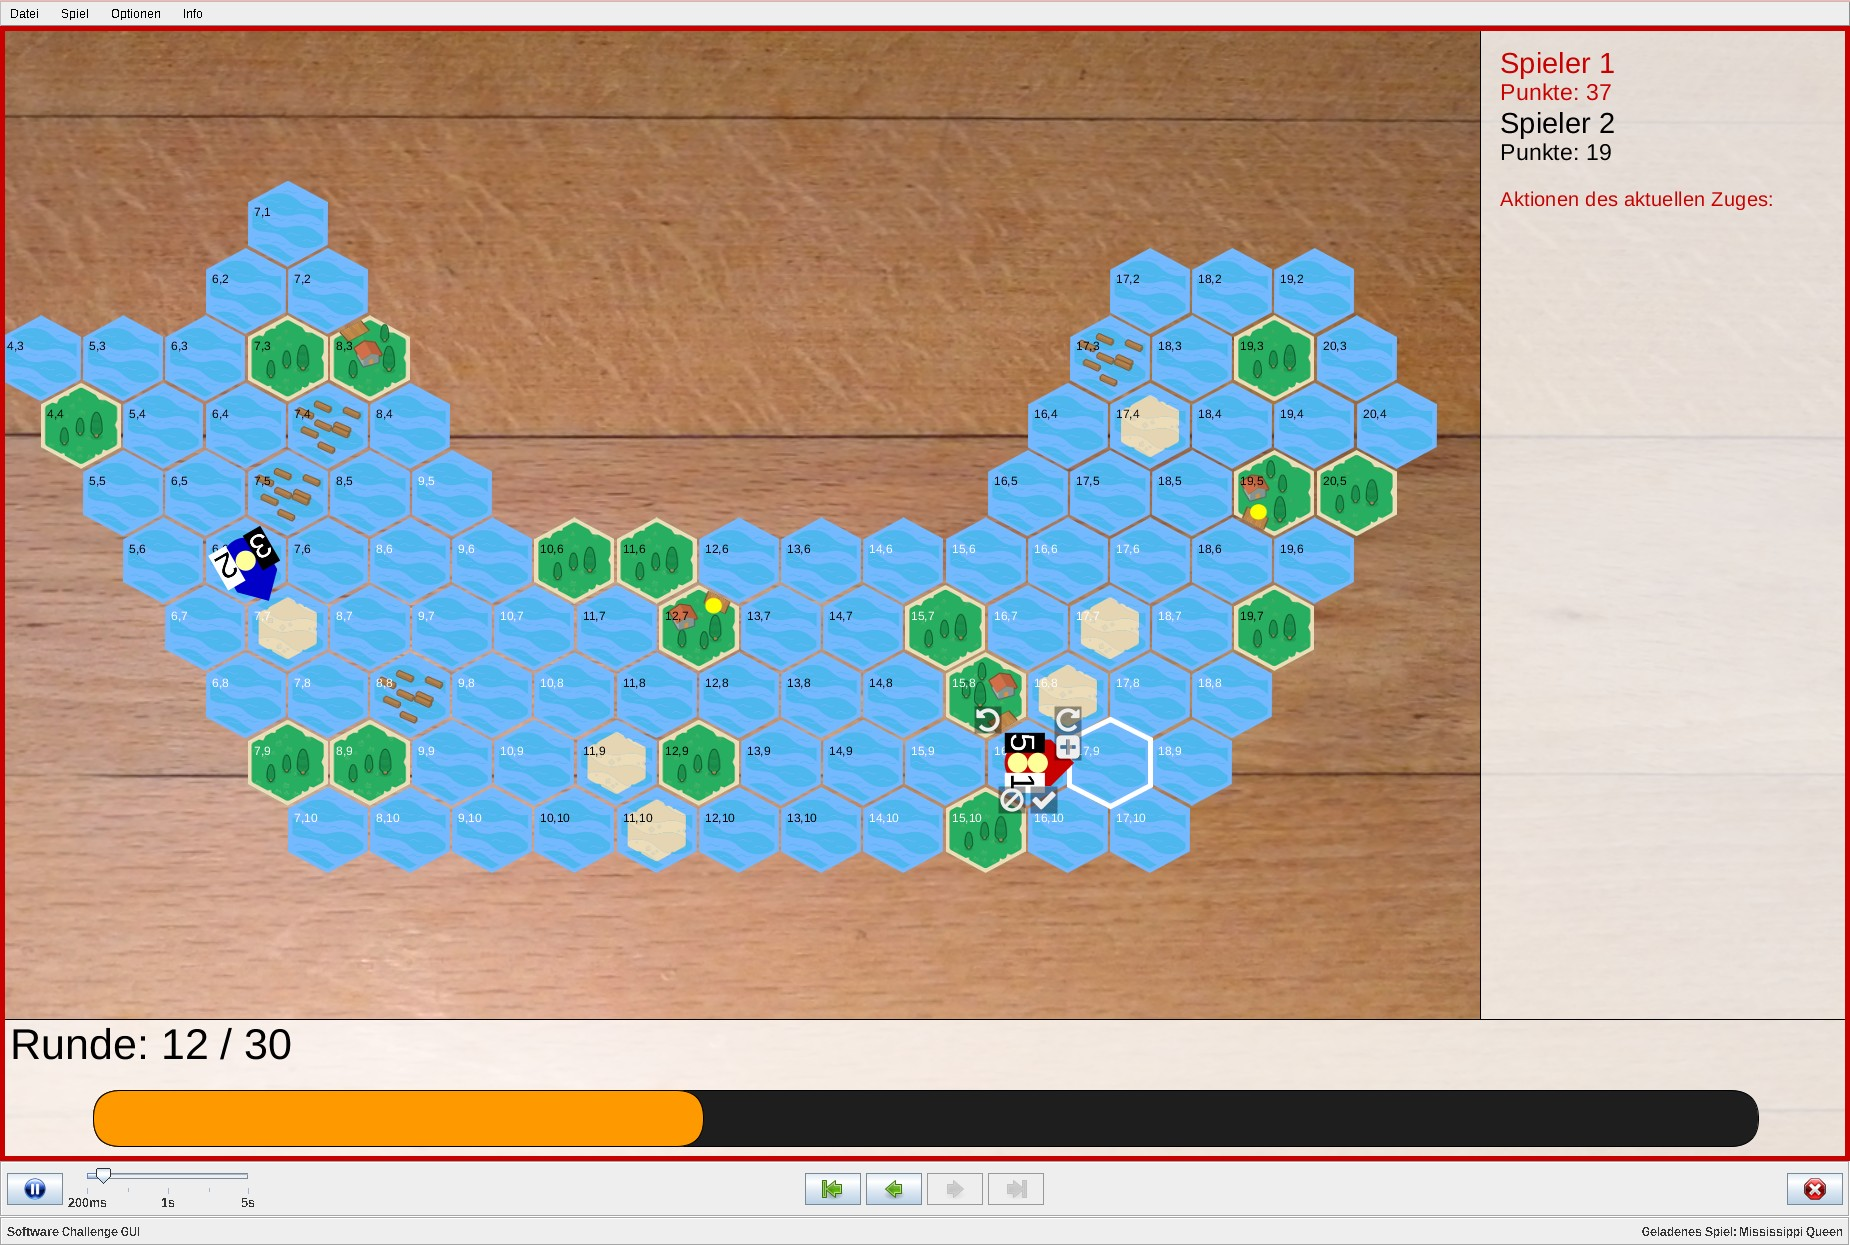
\includegraphics[width=\textwidth]{bilder/spielfeld-gross.jpg}
%\begin{figure}[!htbp]
%  \centering
%  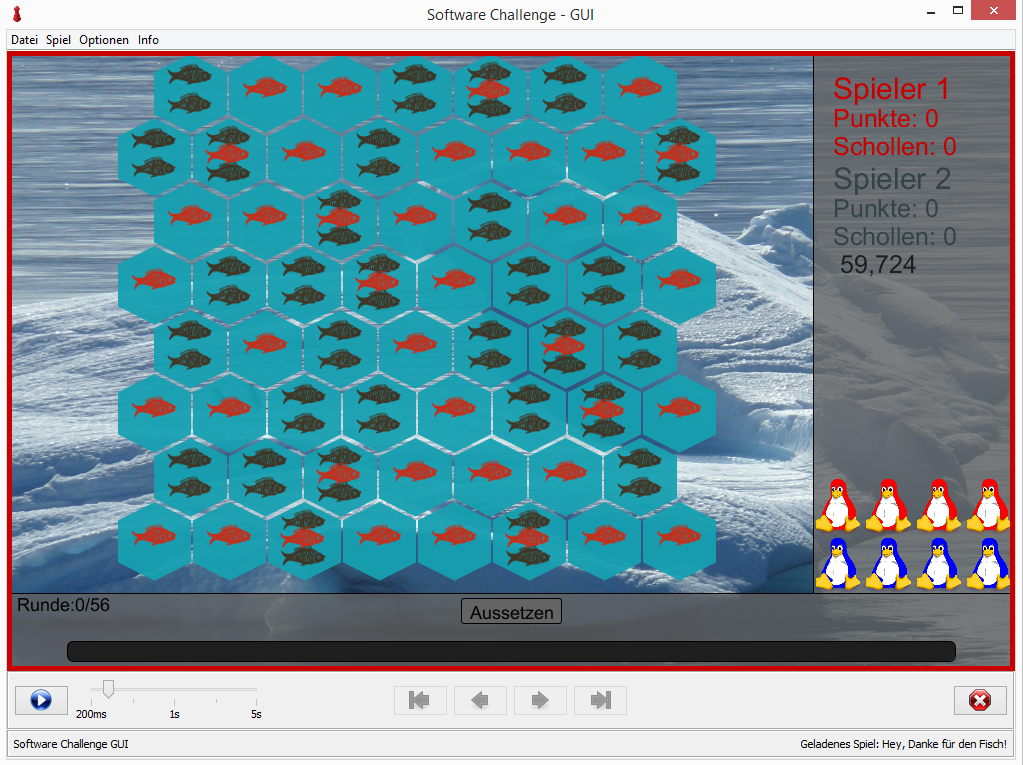
\includegraphics[width=\linewidth]{bilder/gui.png}
%\end{figure}
\vspace*{\fill}

\newpage
\tableofcontents
\thispagestyle{empty}
\newpage
\setcounter{page}{1}

\section{Einleitung}

In dieser Anleitung werden die Elemente und Regeln des Spiels Mississippi Queen
der Software-Challenge 2017 erläutert. Bei Mississippi Queen versuchen zwei
Spieler, durch abwechselndes Setzen von Raddampfern schnellstmöglich einen Fluss
bis zum Ziel entlangzufahren und dabei unterwegs zwei Passagiere mitzunehmen.
Der Spieler dessen Dampfer das Ziel mit zwei Passagieren an Bord zuerst
erreicht, gewinnt das Spiel.


\section{Das Spielbrett}

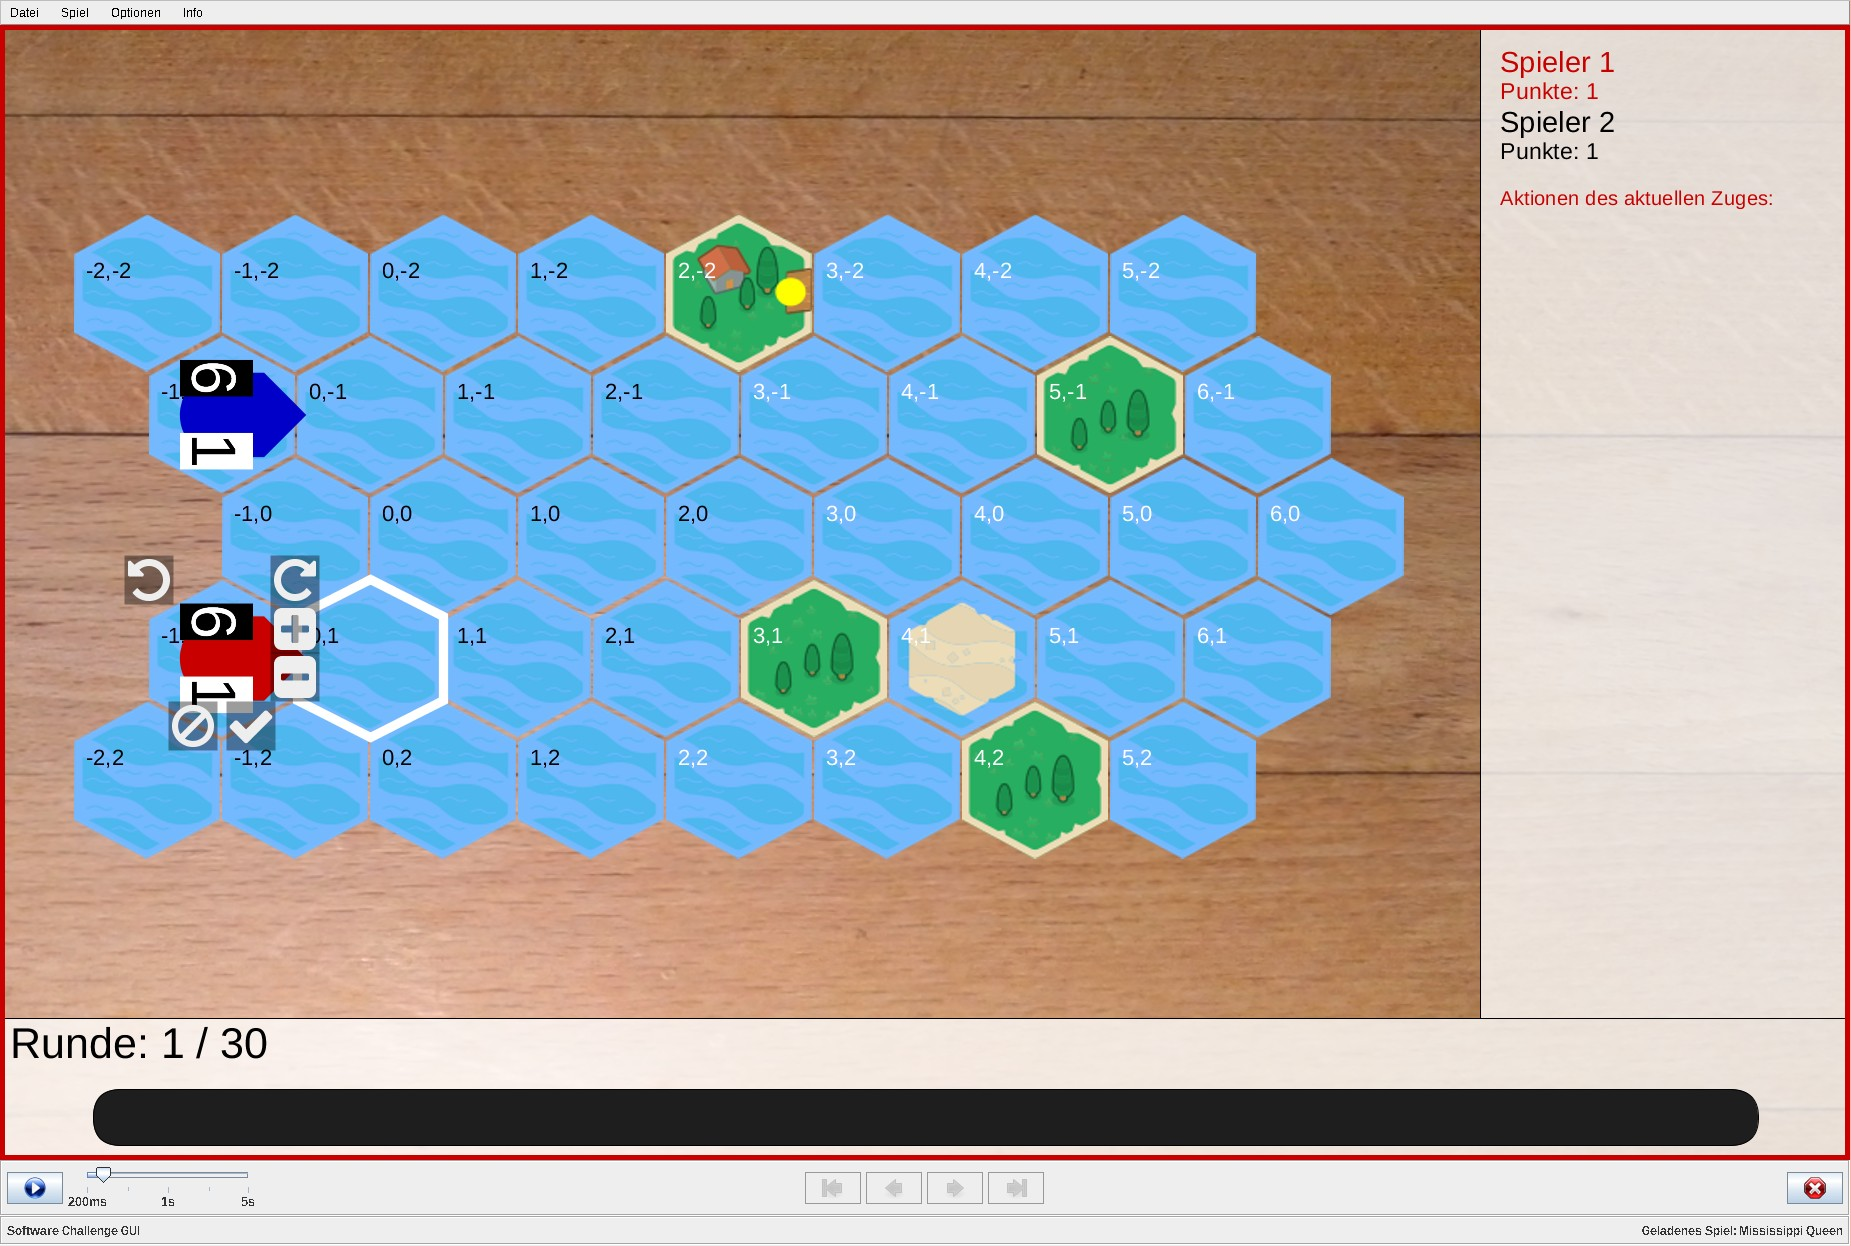
\includegraphics[width=\textwidth]{bilder/spielfeld-anfang.jpg}

Ein mögliches Spielbrett zu Beginn des Spiels sieht man oben. Ein Spielbrett
nachdem das Spiel schon etwas weiter fortgeschritten ist, sieht man auf der
Titelseite dieser Anleitung. Das gesamte Spielbrett besteht aus \Tiles/
Spielsegmenten, mit jeweils \FieldsPerTile/ Feldern. Die Segmente kann durch die
Farbe der Koordinaten auf den Feldern erkennen: Die Segmente haben abwechselnd
schwarze und weiße Koordinaten auf den Feldern. Am Anfang ist nur das
Startsegment und ein darauf folgendes Segment aufgedeckt. Sobald ein Dampfer auf
das zuletzt aufgedeckte Segment fährt, wird ein neues dahinter zufällig links,
rechts oder mittig aufgedeckt. Dies geschieht solange, bis alle \Tiles/ Segmente
aufgedeckt sind. Das letzte Segment ist das Zielsegment (TODO Graphik einfügen
darin Zielfelder markieren). Segmente die schon von allen Spielern betreten und
wieder verlassen wurden, werden vom Spielplan entfernt, auch wenn sich darauf
noch Passagiere befinden.

Die Spielsegmente bestehen aus verschiedene Arten von Hexagon-Feldern, die
zufällig verteilt sind. Neben Wasserfeldern, Inseln, Sandbänken und Baumstämmen
gibt es pro Spiel insgesamt \Passagiere/ Passagierfelder.

Jeder Dampfer beginnt das Spiel mit einer Geschwindigkeit von 1 und einem
Kohlevorrat von 6. Der Dampfer hat außerdem eine von sechs Bewegungsrichtungen,
die den Seiten des Hexagon-Feldes entsprechen, aus denen die Segmente aufgebaut
sind. Die Geschwindigkeit eines Dampfers bestimmt, wie viele Bewegungspunkte er
in einer Runde zur Verfügung hat. Den Kohlevorrat kann man nutzen, um besondere
Aktionen durchzuführen und die Bewegungsrichtung bestimmt, wohin der Dampfer
gerade fährt.

\subsection{\label{water}Das Wasserfeld}

\fieldGraphic{r}{wasser}

Das Wasserfeld kann ganz normal befahren werden. Auf ein zum Spieler in der
aktuellen Bewegungsrichtung benachbartes Wasserfeld ziehen kostet einen
Bewegungspunkt.

\paragraph{}

\subsection{\label{island}Die Insel}

\fieldGraphic{r}{insel}

Die Insel kann nicht überquert werden. Fährt ein Dampfer auf eine Insel (z.B.
weil er nicht rechtzeitig bremsen kann) hat er das Spiel verloren.

\paragraph{}

\subsection{\label{passenger}Das Passagierfeld mit Anleger in Richtung $i$}

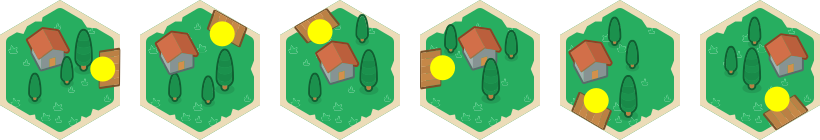
\includegraphics[width=\textwidth]{bilder/passagier}

Auf dem Passagierfeld mit Anleger in Richtung $i$ wartet eine Passagier, der am
Anleger abgeholt werden kann. Um den Passagier abzuholen, muss
der Dampfer mit Geschwindigkeit 1 am Anleger ankommen. Es verwandelt sich in ein normales
Inselfeld, sobald der Passagier abgeholt wurde (siehe Insel, \ref{island}).


\subsection{\label{sandbank}Die Sandbank}

\fieldGraphic{r}{sandbank}

Eine Sandbank stoppt einen Dampfer, sollte er darauf fahren. Das heißt wenn ein
Spieler auf eine Sandbank fährt, beendet dies seinen Zug und setzt seine
Geschwindigkeit auf 1. Es kann im nächsten Zug nur rückwärts oder vorwärts mit
der Bewegungsrichtung, mit der die Sandbank befahren wurde, wieder verlassen werden.
Verlässt man es Rückwärts, kostet dies zusätzlich eine Kohleeinheit. Auf einer
Sandbank kann nicht gedreht werden und ein Dampfer, der sich darauf befindet,
kann nicht abgedrängt werden.

\paragraph{}

\subsection{Das Baumstammfeld}

\fieldGraphic{r}{baumstaemme}

Das ziehen in ein Baumstammfeld kostet zwei Bewegungspunkte statt einem.
Außerdem wird die Geschwindigkeit eines Schiffes, welches ein Baumstammfeld
durchquert nach dem Zug um 1 verringert. Sind nicht genug Bewegungspunkte
vorhanden, kann es nicht überquert werden. Das Abdrängen in ein Baumstammfeld
kostet einen zusätzlichen Bewegungspunkt.

\paragraph{}

\subsection{\label{goal}Das Zielfeld}

\fieldGraphic{r}{ziel}

Ein Zielfeld ist ein Feld, das erreicht werden kann, um das Spiel zu gewinnen.
Ein Zielfeld muss mit Geschwindigkeit 1 befahren werden und es müssen sich zwei
Passagiere an Bord befinden, damit der Dampfer das Spiel gewinnt. Sind diese
Bedingungen nicht erfüllt, kann ein Zielfeld wie ein Wasserfeld befahren werden.

\paragraph{}

\section{Spielablauf}

Beide Spieler starten mit Geschwindigkeit 1 und 6 Kohleeinheiten und ziehen dann
abwechselnd. Ein Zug besteht aus einer oder mehreren Aktionen. In einem Zug
müssen (falls der Zug nicht auf einer Sandbank endet) durch die Aktionen
insgesamt alle Bewegungspunkte (bestimmt durch die Geschwindigkeit des Schiffes)
verbraucht werden. Die verschiedenen Aktionen sind:


\subsection{\label{acceleration}Beschleunigungsaktion}

Eine Beschleunigung Kann nur als erste Aktion eines Zuges ausgeführt werden. Die
Beschleunigung um eine Geschwindigkeitseinheit pro Zug ist frei, jede
Beschleunigung um mehr als 1 kostet für jeden weiteren Geschwindigkeitspunkt
eine Kohleeinheit. Möchte ein Spieler beispielsweise mit einer aktuellen
Geschwindigkeit von 2 auf Geschwindigkeit 4 beschleunigen, kostet dies eine
Kohleeinheit. Die maximale Geschwindigkeit ist 6, die niedrigste 1. Eine
Beschleunigungsaktion um 0 ist ungültig. Es ist aber zulässig, keine
Beschleunigungsaktion durchzuführen und so die Geschwindigkeit beizubehalten.

Auf gleiche weise kann auch abgebremst, also die Geschwindigkeit verringert
werden. Dies wird der Einfachheit halber als Beschleunigungsaktion mit negativer
Beschleunigung behandelt.

\subsection{Erzeugung der Bewegungspunkte}

Bevor nun eine der folgenden Aktionen durchgeführt werden kann, bekommt der
Dampfer entsprechend seiner aktuellen Geschwindigkeit Bewegungspunkte. Diese
Bewegungspunkte müssen durch die folgenden Aktionen aufgebraucht werden, am Ende
des Zuges dürfen also keine Bewegungspunkte mehr vorhanden sein.

\subsection{\label{turn}Drehaktion}

Eine Drehaktion je Zug des Spielers um eine Einheit (also um 60\degree) ist frei
(Ausnahme Abdrängen, siehe \ref{push}). Jede weitere Drehung erfordert eine
Kohleeinheit. Es kann sich nicht auf Sandbänken gedreht werden.


\subsection{\label{push}Abdrängaktion}

Endet eine Aktion auf einem Feld mit dem gegnerischen Dampfer, muss darauf eine
Abdrängaktion folgen. Ein Spieler kann den Gegner auf ein beliebig angrenzendes,
jedoch nicht direkt hinter dem Spieler liegendes, begehbares Feld abdrängen
(\label{passierbar}Wasserfelder, Sändbänke und Baumstammfelder gelten als
begehbar). Eine Abdrängaktion kostet einen Bewegungspunkt, zwei, falls auf ein
Baumstammfeld abgedrängt wird. Es darf nicht von einer Sandbank aus abgedrängt
werden. Der abgedrängte Spieler bekommt eine zusätzliche freie Drehung für
seinen nächsten Zug. Wurde der Spieler auf eine Sandbank abgedrängt, entfällt
diese freie Drehung und die Geschwindigkeit des abgedrängten Spielers wird auf 1
reduziert.

\subsection{\label{step}Bewegungsaktion}

Eine Bewegungsaktion erfolgt in die derzeitige Bewegungsrichtung des Schiffes.
Sie kann nur über und auf passierbare (siehe \ref{passierbar}) Felder erfolgen.
Sie darf niemals durch ein vom Gegner besetztes Feld oder eine Sandbank gehen,
darf auf dem Feld des Gegners oder einer Sandbank enden.

\subsection{Kombination von Aktionen}

Solange die Regeln der einzelnen Aktionsarten eingehalten werden, können mehrere
Aktionen innerhalb eines Zuges beliebig kombiniert werden.

\section{Spielende}

\begin{centering}
  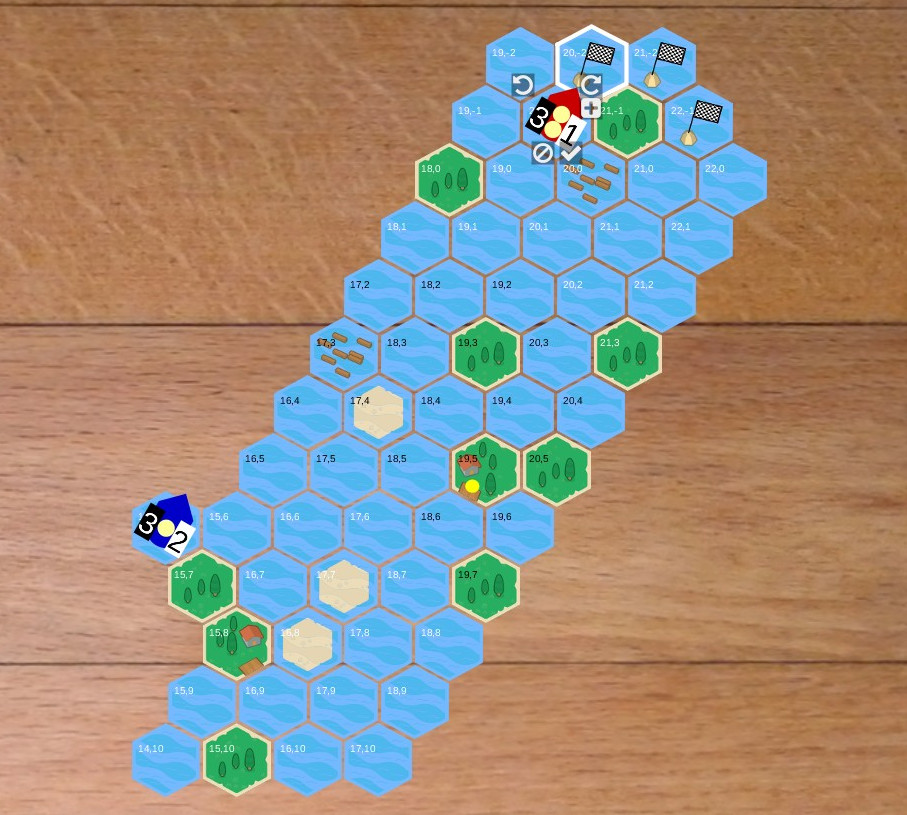
\includegraphics[width=\textwidth]{bilder/spielfeld-ziel.jpg}
\end{centering}

Das Spiel ist beendet, sobald

\begin{itemize}
\item ein Dampfer mit 2 Passagieren ein Zielfeld mit Geschwindigkeit 1 erreicht hat.
\item ein Spieler einen unültigen Zug macht.
\item am Ende einer Runder ein Dampfer mehr als 3 Spielsegmente zurückliegt.
  \item das Rundenlimit von 30 Runden erreicht ist.
\end{itemize}

Ein Spieler, der einen ungültigen Zug macht, erhält für das Spiel insgesamt 0
Punkte. In allen anderen Fällen berechnet sich der Punktestand eines jeden
Spielers folgendermaßen:

\begin{itemize}
  \item Jeder eingesammelte Passagier bringt 5 Punkte
  \item Jedes überwundene Segment bringt 5 Punkte.
  \item Anhand der Position innerhalb eines Segments werden 0 bis 4 Punkte
    vergeben. (Ein Segment ist aufgeteilt in 5 Reihen. Je weiter vorne man ist,
    desto mehr Punkte bekommt man TODO siehe Graphik).
\end{itemize}

Bei Spielende gewinnt der Spieler mit den meisten Punkten. Sollten beide Spieler
gleich viele Punkte haben, gewinnt der Spieler, der mehr Passagiere eingesammelt
hat. Sollte auch diese Zahl gleich sein, endet das Spiel unentschieden.

\section{Die graphische Benutzeroberfläche für menschliche Spieler}

Über die grafische Benutzeroberfläche (auch GUI Server genannt) können zwei
menschliche Spieler gegeneinander oder ein menschlicher Spieler gegen einen
Computerspieler spielen (ausserdem kann man Spielaufzeichnungen abspielen und
Massentests von Computerspielern durchführen).

Die Bedienung des Spiels durch einen menschlichen Spieler wird im Folgenden
erklärt.

\subsection{Neues Spiel starten}

TODO

\subsection{Hauptbildschirm}

\begin{centering}
  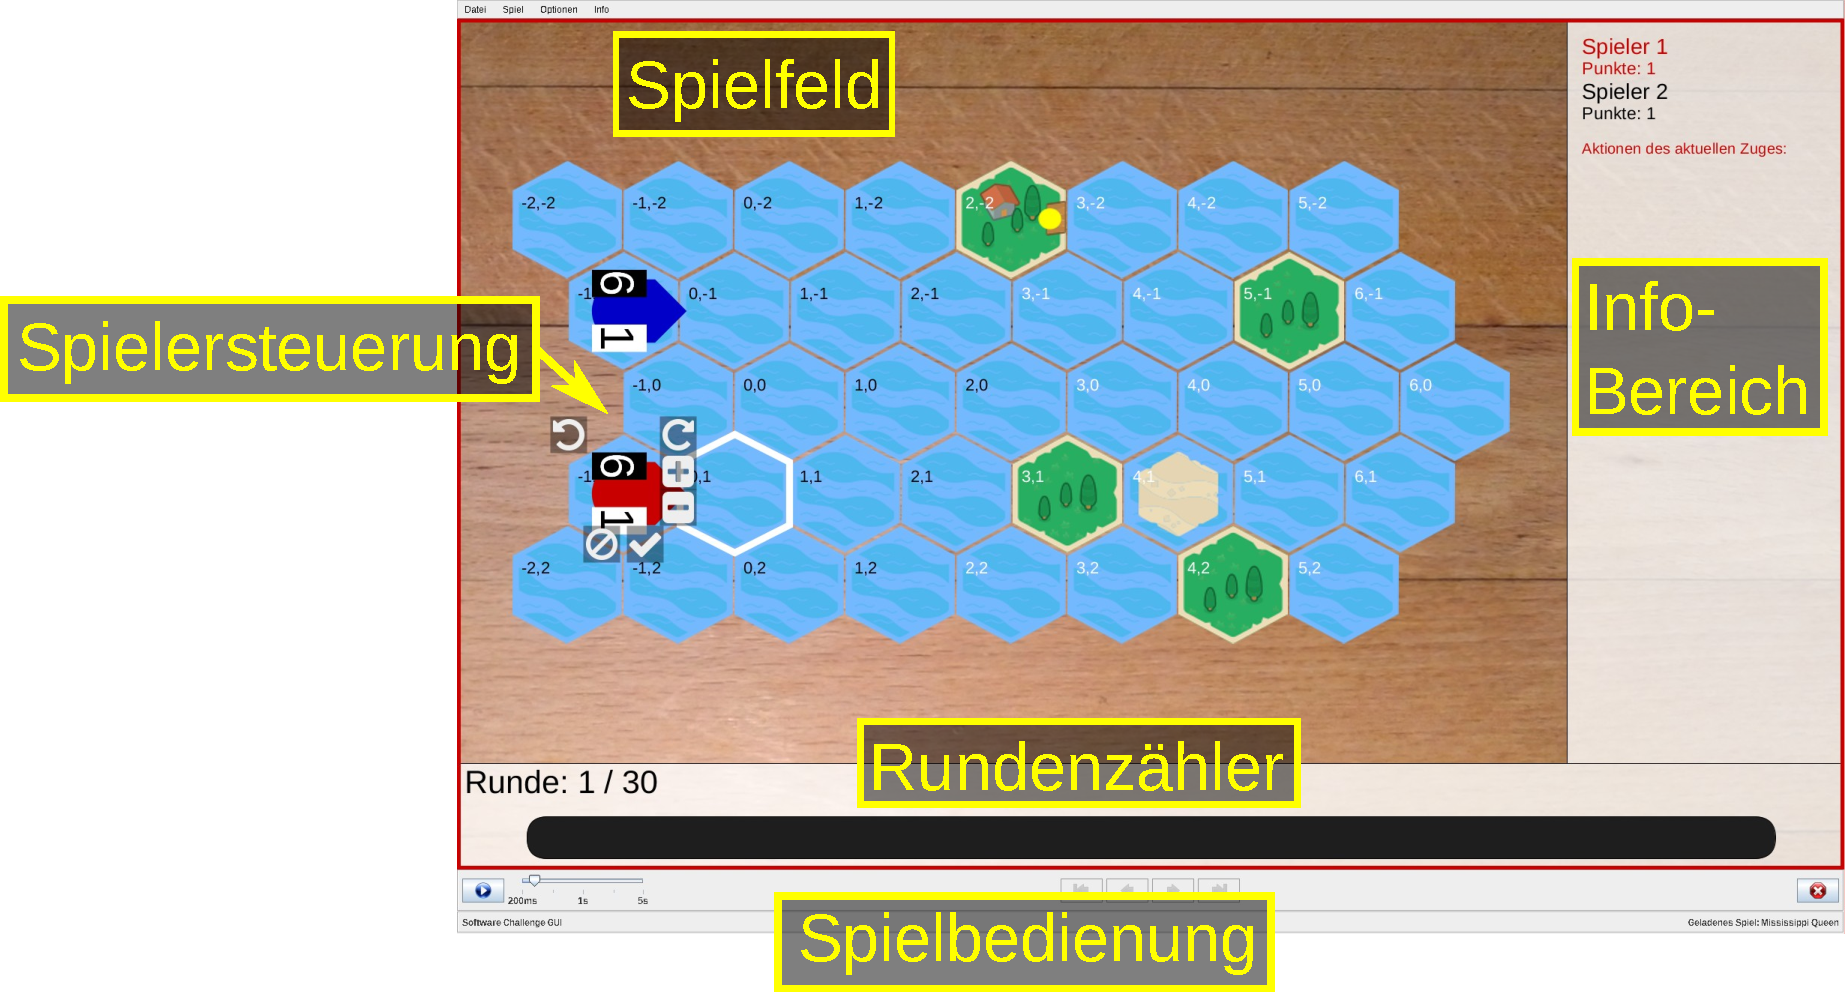
\includegraphics[width=\textwidth]{bilder/gui-elemente.pdf}
\end{centering}

In der obigen Abbildung sind die Grundelemente der grafischen Oberfläche des
Spiels dargestellt und beschriftet. Der Hauptbereich besteht aus der Darstellung
des Spielfeldes in das Spielfeld eingebettet sind ist die Spielsteuerung, falls
gerade ein menschlicher Spieler am Zug ist. Rechts vom Hauptbereich befindet
sich ein Info-Bereich, in dem die Spielernamen, die bisher erreichten Punkte der
Spieler sowie die bisher gemachten Aktionen eines menschlichen Spielers im
aktuellen Zug textuell dargestellt werden. Unterhalb des Hauptbereichs und des
Info-Bereichs befindet sich der Rundenzähler, auf dem man die aktuelle Runde
ablesen kann. Darunter findet man die Bedienelemente zum kontrollieren des
Spielablaufes, die Spielbedienung.

\subsection{Spielsteuerung}

Wenn ein menschlicher Spieler am Zug ist, kann er die Aktionen, die er in seinem
Zug durchführen will, über die Spielsteuerung eingeben. Die Spielsteuerung
besteht aus bis zu sechs Icons, die neben dem Dampfer des Spielers dargestellt
werden, sowie eventuell ein oder mehreren weiß umrandeten Hexagonal-Feldern.
Durch Klicken auf ein Spielsteuerungselement wird die damit verbundene Aktion
ausgelöst. Die Aktionen sind im einzelnen:

\begin{table}[h!]
  \centering
  \begin{tabular}{ c m{0.7\linewidth} }
    Element & Beschreibung \\
    \hline
    \begin{minipage}{1cm}
      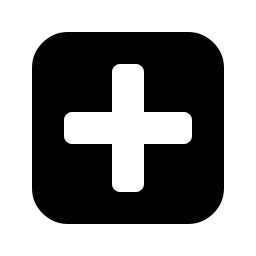
\includegraphics[width=\linewidth]{bilder/plus-square}
    \end{minipage}
    &
    Beschleunigung um 1. Wenn um mehr als 1 beschleunigt werden soll, entsprechend oft hintereinander anklicken. Beschleunigung ist nur als erste Aktion verfügbar.
    \\
    \begin{minipage}{1cm}
      
\includegraphics[width=\linewidth]{bilder/minus-square}
    \end{minipage}
    &
    Abbremsen um 1. Wenn um mehr als 1 abgebremst werden soll, entsprechend oft hintereinander anklicken. Abbremsen ist nur als erste Aktion verfügbar.
    \\
    \begin{minipage}{1cm}
      
\includegraphics[width=\linewidth]{bilder/rotate-left}
    \end{minipage}
    &
    Drehung um eine Einheit nach links.
    \\
    \begin{minipage}{1cm}
      
\includegraphics[width=\linewidth]{bilder/rotate-right}
    \end{minipage}
    &
    Drehung um eine Einheit nach rechts.
    \\
    \begin{minipage}{1cm}
      
\includegraphics[width=\linewidth]{bilder/rotate-right}
    \end{minipage}
    &
    Drehung um eine Einheit nach rechts.
    \\
    \begin{minipage}{1cm}
      
\includegraphics[width=\linewidth]{bilder/okay}
    \end{minipage}
    &
    Zug ist vollständig. Falls der eingegebene Zug ungültig ist, erscheint
    eine Sicherheitsabfrage, ob man den Zug wirklich so durchführen möchte (was
    bei ungültigen Zügen zu einer Disqualifikation führt).
    \\
    \begin{minipage}{1cm}
      
\includegraphics[width=\linewidth]{bilder/cancel}
    \end{minipage}
    &
    Bisher eingegebene Aktionen löschen und von vorn mit der Eingabe beginnen.
    \\
    \begin{minipage}{1cm}
      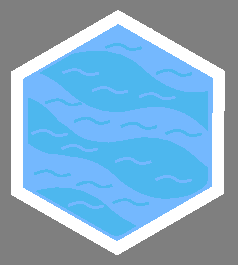
\includegraphics[width=\linewidth]{bilder/water-marked}
    \end{minipage}
    &
    Bewegung auf dieses Feld oder im Fall einer Abdrängaktion (siehe \ref{sec:push}): Abdrängen des Gegners auf dieses Feld.
  \end{tabular}
\end{table}

\subsection{Abdrängen}\label{sec:push}

\begin{centering}
  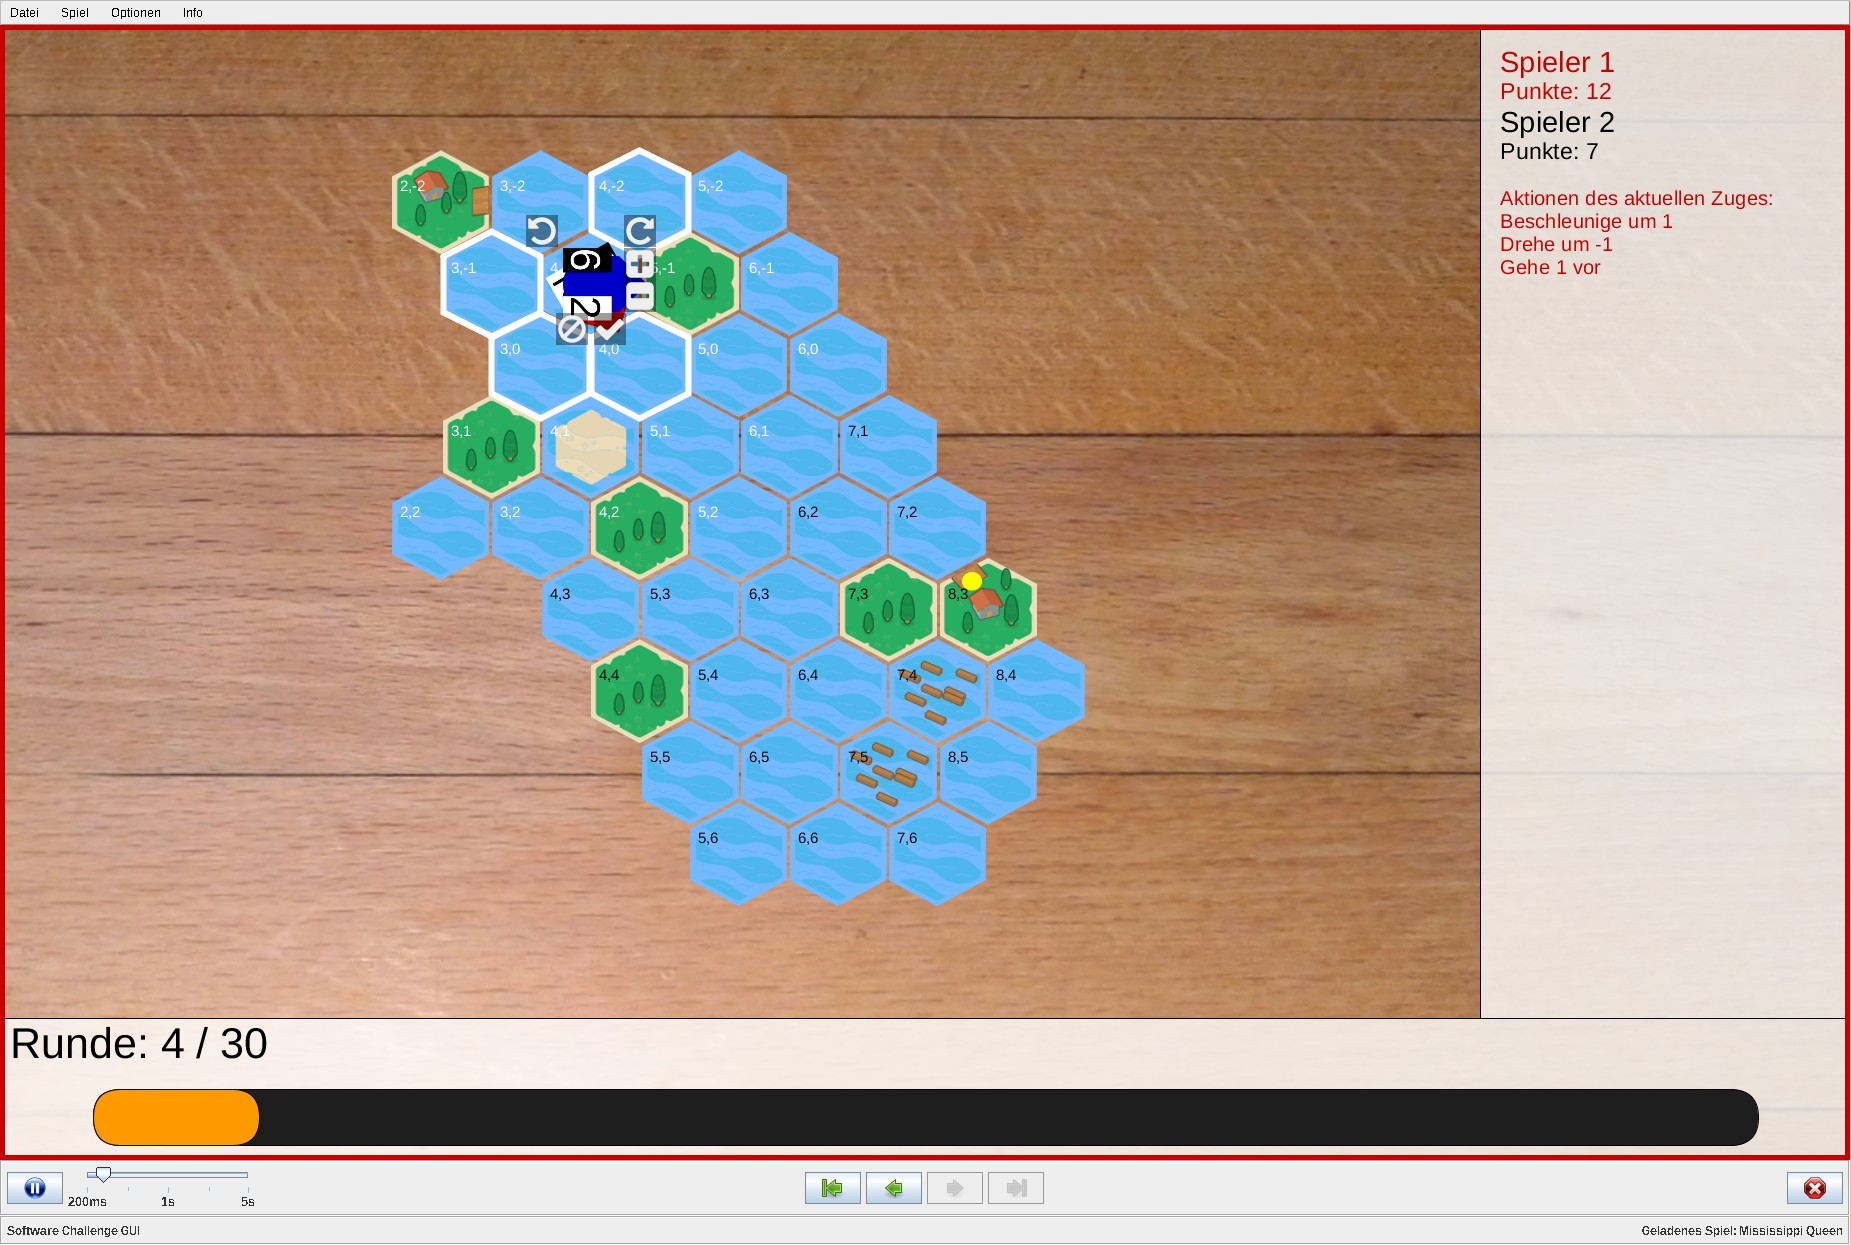
\includegraphics[width=\textwidth]{bilder/spielfeld-abdraengen.jpg}
\end{centering}

TODO

\subsection{Passagiere aufnehmen}

TODO

\subsection{Spielbedienung}

TODO

\end{document}
